\section{Evaluación y Corrección de Estacionariedad}

Al igual que el modelo de Holt-Winters, el modelo de Arima también requiere que los datos sean estacionarios, es decir, qeu su media y varianza sean constantes en el tiempo. 

Para verificar esto se pueden hacer dos pruebas estadísticas: Augmented Dickey-Füller Test(ADF) y Kwiatkowski-Phillips-Schmidt-Shin Test(KPSS).\\

La primera tiene la hipótesis Nula, que la serie no es estacionaria, y por lo tanto si el $p-value$ es menor a 0,05 es rechazada y la serie es estacionaria.\\

La segunda tiene como hipótesis Nula, que la serie es estacionaria.
Si aplicamos el siguiente código, obtenemos el resultado de la siguiente figura que resume los resultados del código.\\

\begin{lstlisting}
	datos_diff_1 = datos.diff(1).dropna()
	print('Test estacionariedad serie original')
	print(f'ADF Statistic: {adfuller(datos)[0]}, p-value: {adfuller(datos)[1]}')
	print(f'KPSS Statistic: {kpss(datos)[0]}, p-value: {kpss(datos)[1]}')
	print('\nTest estacionariedad serie diferenciada de orden 1')
	print(f'ADF Statistic:
	 {adfuller(datos_diff_1)[0]}, p-value: {adfuller(datos_diff_1)[1]}')
	print(f'KPSS Statistic:
	 {kpss(datos_diff_1)[0]}, p-value: {kpss(datos_diff_1)[1]}')
\end{lstlisting}


\begin{figure}[h]
	\centering
	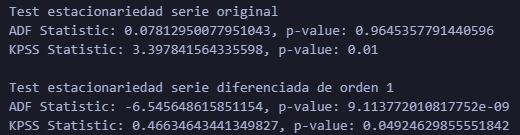
\includegraphics[width=0.7\linewidth]{fuller}
	\caption{ADF y KPSS orden 1}
	\label{fig:fuller}
\end{figure}

\textbf{Conclusiones}:
\begin{enumerate}
	\item Serie Original:
	\begin{itemize}
		\item ADF Statistic = 0.0781, p-value = 0.9645. No se rechaza Hipótesis Nula, lo que indica que la serie no es estacionaria.
		\item KPSS Statistic = 3.3978, p-value = 0.01.  Se rechaza Hipótesis Nula, lo que confirma que la serie no es estacionaria.
	\end{itemize}
	\item Serie Diferenciada:
	\begin{itemize}
		\item ADF Statistic = -6.5456, p-value = 9.11e-09. Se rechaza Hipótesis Nula, lo que indica que la serie ahora es estacionaria.
		\item KPSS Statistic = 0.4663, p-value = 0.0492. No se rechaza Hipótesis Nula, lo que confirma que la serie es estacionaria.
	\end{itemize}
\end{enumerate}

Una vez transformada la serie a estacionaria se puede empezar el análisis de autocorrelación.

\section{Autocorrelación}

Se distingue entre la autocorrelación simple (ACF) y parcial (PACF).

La autocorrelación ACF ayuda a identificar si una serie es o no estacionaria, mientras que la parcial PACF ayuda a identificar el modelo autorregresivo a utilizar.

\begin{figure}[h]
	\centering
	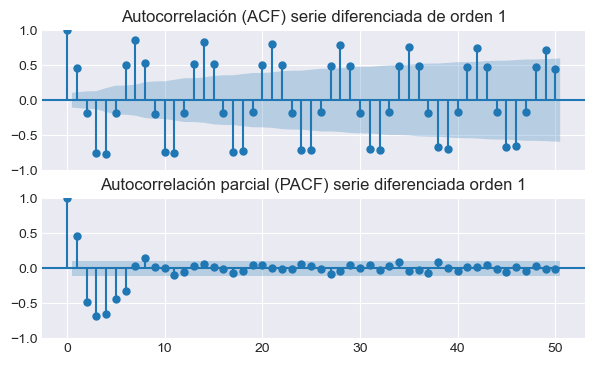
\includegraphics[width=0.7\linewidth]{autocorrelacion_PACF_ACF}
	\caption{Autocorrelación ACF y PACF orden 1}
	\label{fig:autocorrelacionpacfacf}
\end{figure}

\textbf{Análisis del gráfico superior:}
\begin{itemize}
	\item Presenta una disminución lenta de la autocorrelación, pero aún se observan algunos valores altos.
	\item Esto sugiere que la serie aún puede tener cierta estructura de dependencia en el tiempo, lo que indica que la diferenciación puede no haber sido suficiente o que la serie tiene una componente de media móvil. 
\end{itemize}

\textbf{Análisis del gráfico inferior:}
\begin{itemize}
	\item Muestra un corte brusco después de los primeros rezagos, lo cual es característico de un proceso AR(p).
	\item  La presencia de valores significativos en los primeros rezagos indica que la serie podría ser modelada con un proceso ARMA o ARIMA con un componente autorregresivo.
\end{itemize}

Se obtienen las siguientes conclusiones de las autocorrelaciones:
\begin{itemize}
	\item La ACF muestra una disminución lente, lo que puede indicar que un modelo MAq o un modelo mixto ARMA sería adecuado.
	\item La PACF apunta a un modelo ARIMA con un componente AR de bajo orden.

\end{itemize}
Conclusiones preliminares:
La serie ya ha sido diferenciada una vez, lo que sugiere que podría haber sido originalmente no estacionaria.
La ACF muestra una disminución lenta, lo que podría indicar que un modelo MA(q) o un modelo mixto ARMA sería adecuado.

\subsection{Serie Diferencia Orden 1}

Para poder seleccionar el modelo, primero se integrará la descomposición con el análisis de ACF y PACF previamente hecho.
Esto permitirá hacer una descripción integral que ayude a comprender la estructura subyacente de los datos y a determinar los valores óptimos de los parámetors ARIMA.

De la siguiente figura se puede observar lo siguiente:

\begin{enumerate}
	\item	Serie Observada
	\begin{itemize}
		\item Se ve una fuerte estacionalidad y fluctuaciones regulares
	\end{itemize}
	\item Tendencia
	\begin{itemize}
		\item No se aprecia una tendencia clara, es bastante errática, esto indica que la diferenciación ya eliminó cualquier tendencia significativa.
	\end{itemize}
	\item Estacionalidad
	\begin{itemize}
		\item Presenta patrones repetitivos en intervalos regulares.
		\item  La serie sigue teniendo una fuerte estacionalidad, lo que indica que la diferenciación de primer orden no eliminó por completo la componente estacional. Para modelar con ARIMA es necesario aplicar otra diferenciación.
	\end{itemize}
	\item Residuo
	\begin{itemize}
		\item Se ven ciertas fluctuaciones y correlaciones, lo que sugiere que aún hay información en la serie que podría ser modelada con ARMA o ARIMA.		
	\end{itemize}
\end{enumerate}

\begin{figure}[h]
	\centering
	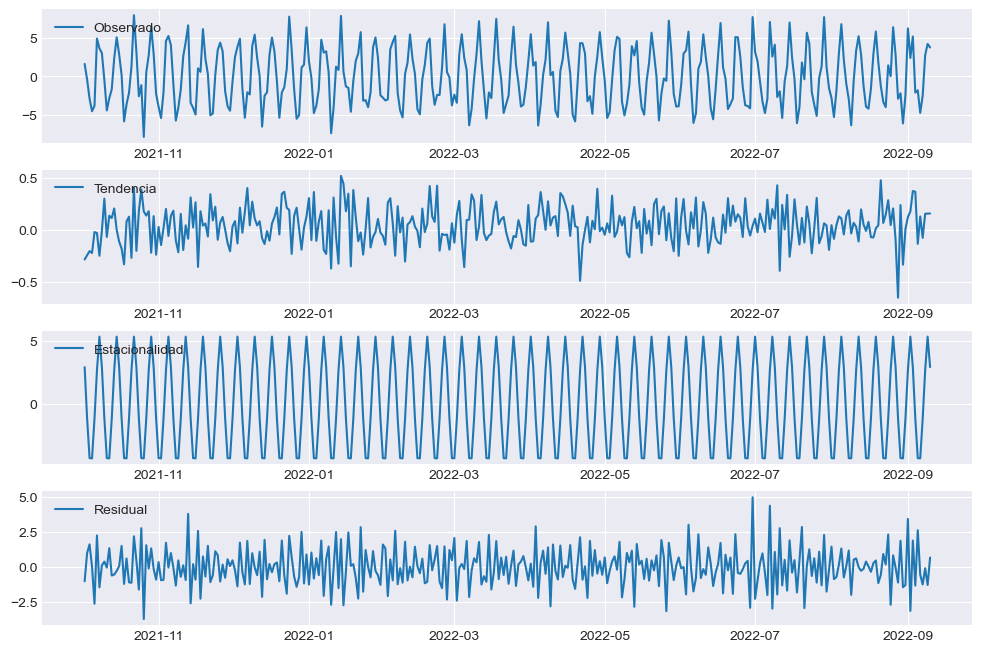
\includegraphics[width=0.7\linewidth]{seasonal_decompose_plot_diff}
	\caption{Descomposicion Estacional orden 1}
	\label{fig:seasonaldecomposeplotdiff}
\end{figure}


\subsection{Serie Diferenciada Orden 7}
Se decide aplicar la función de autocorrelación (ACF) y autocorrelación parcial (PACF) sobre una serie diferenciada de orden 7, debido a que la estacionalidad observada parece repetirse semanalmente.

\begin{lstlisting}
	datos_diff_1_7 = datos_diff_1.diff(7).dropna()
	print('Test estacionariedad serie de orden 7')
	print('\nTest estacionariedad serie diferenciada de orden 7')
	print(f'ADF Statistic: {adfuller(datos_diff_1_7)[0]}, p-value: {adfuller(datos_diff_1_7)[1]}')
	print(f'KPSS Statistic: {kpss(datos_diff_1_7)[0]}, p-value: {kpss(datos_diff_1_7)[1]}')
\end{lstlisting}

Los resultados de los tests de estacionariedad muestran que la serie es estacionaria.
\begin{figure}[h]
	\centering
	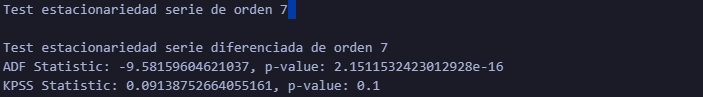
\includegraphics[width=0.7\linewidth]{orden7_fuller}
	\caption{Resultados ADF y KPSS orden 7}
	\label{fig:orden7fuller}
\end{figure}

En la siguiente figura se observa que la estacionalidad se ha reducido, la tendencia es más estable y los residuos muestran un comportamiento más aleatorio que antes.
Dado que la componente estacional aún persiste, un modelo SARIMA con $D = 1$ podría ser una opción adecuada.

\begin{figure}[h]
	\centering
	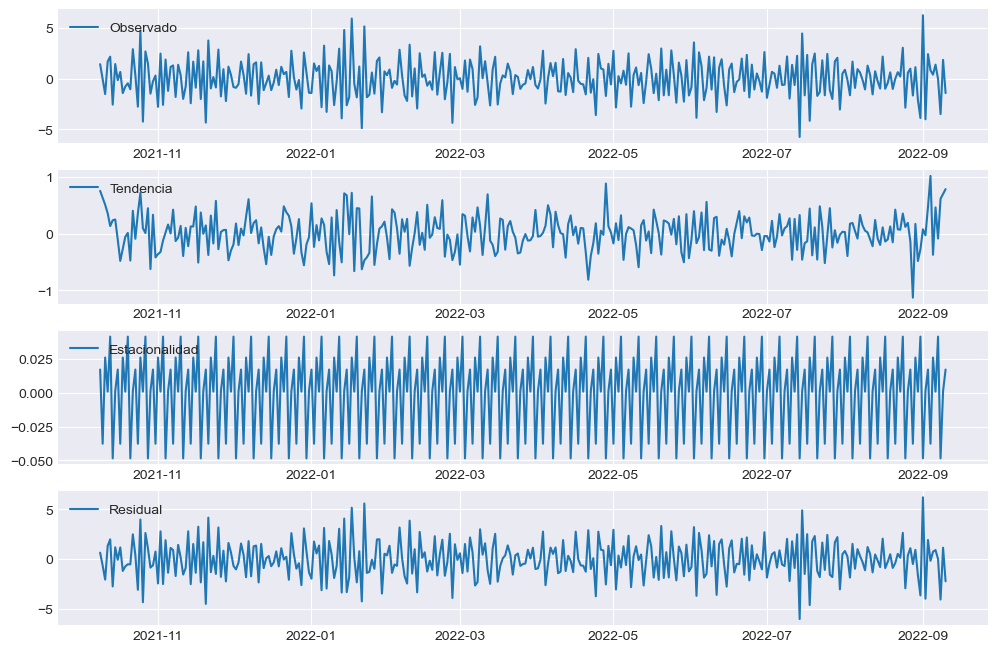
\includegraphics[width=0.7\linewidth]{seasonal_decompose_plot_diff_7}
	\caption{Descomposicion Estacional orden 7}
	\label{fig:seasonaldecomposeplotdiff7}
\end{figure}

\subsection{Autocorrelación de la Serie Diferenciada de Orden 7}
La siguiente figura muestra la función de autocorrelación y autocorrelación parcial aplicadas a la serie diferenciada de orden 7. 

\begin{figure}[h]
	\centering
	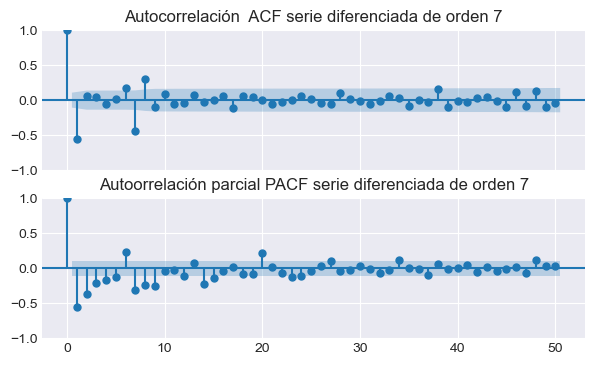
\includegraphics[width=0.7\linewidth]{dif7_autocorrelacion_PACF_ACF}
	\caption{Autocorrelación ACF y PACF orden 7}
	\label{fig:dif7autocorrelacionpacfacf}
\end{figure}

\begin{itemize}
\item La serie es estacionaria tras aplicar una diferenciación de orden 7, por lo que se establece $d = 1$ y $D = 1$ para eliminar la tendencia y la estacionalidad semanal.
\item El PACF muestra un corte significativo en el lag 1, lo que sugiere un orden autoregresivo de $p = 1$. También se observa un pico en el lag 7, lo que justifica la elección de $P = 1$.
\item El ACF decrece rápidamente después del primer lag y oscila cerca de 0, lo que sugiere $q = 1$. Al igual que en PACF, se detecta un pico en el lag 7, por lo que se establece $Q = 1$.
\end{itemize}

\section{Modelo SARIMAX}

Para la creación del modelo los valores utilizados serán los siguientes:
\begin{itemize}
	\item $d = 1$, $D = 1$. Para eliminar tendencia y estacionalidad.
	\item $p = 1$, $P = 1$. Basado en la ACF y PACF.
	\item $q = 1$, $Q = 1$ Basado en la ACF y PACF en los lags estacionales (s = 7).
\end{itemize}

Se insertan en el código. Los parámetros en la función SARIMAX, son los antes mecionados.  En la función \lstinline|acorr_ljungbox| se utilizan lags 7, 14 y 50. El primero representa la estacionalidad en 7 días, el segundo el doble del período estacional y el último la cantidad de lags utilizados para la autocorrelación.

La expresión algebraica para representar SARIMAX(1,1,1)(1,1,1,7) sería:

\begin{equation}[h]
	(1 - \phi_1L)\cdot(1 - \Phi_1L^7)\cdot(1 - L)Y_t = (1 - \theta_1L)\cdot(1 - \Theta_1L^7)\cdot \epsilon_t
\end{equation}

De tu salida de SARIMAX Results:
\begin{itemize}
	\item $L$ equivale al operador.
	\item $\epsilon_t$ es un error aleatorio.
	\item $\phi_1 = -0.1192$. Coeficiente del término autorregresivo (AR)
	\item $\Phi_1 = 0.0890$. Coeficiente de la parte estacional autorregresiva (SAR).
	\item $\theta_1 = -0.9317$. Coeficiente del término de media móvil (MA).
	\item $\Theta$ = (-) 0.997 Coeficiente de la parte estacional de media móvil (SMA).
\end{itemize}
	 
\begin{lstlisting}
	warnings.filterwarnings("ignore", category=UserWarning,
	message='Non-invertible|Non-stationary')
	modelo = SARIMAX(endog = train, order = 
	(1, 1, 1), seasonal_order = (1, 1, 1, 7))
	modelo_res = modelo.fit(disp=0)
	warnings.filterwarnings("default")
	modelo_res.summary()
	from statsmodels.stats.diagnostic import acorr_ljungbox
	estadistico_lb, p_valor_lb = acorr_ljungbox
	(modelo_res.resid, lags=[7, 14, 50])
\end{lstlisting}

\begin{figure}[!h]
	\centering
	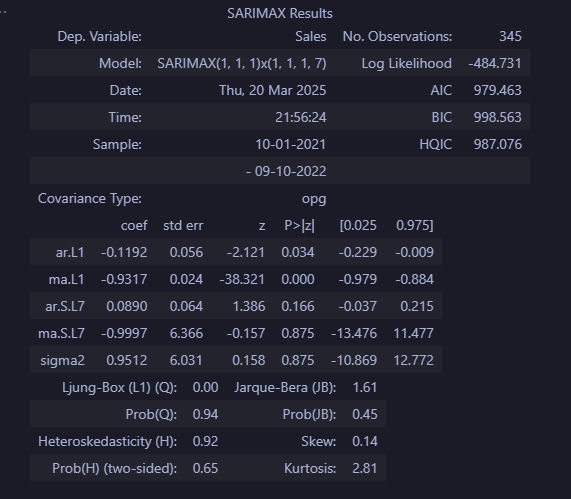
\includegraphics[width=0.5\linewidth]{sarimax_resultados}
	\caption{Resultados Arima Manual}
	\label{fig:sarimaxresultados}
\end{figure}

\begin{lstlisting}
	predicciones = modelo_res.get_forecast(steps=20)
	predicciones_statsmodels = predicciones.predicted_mean
	intervalo_conf = predicciones.conf_int(alpha=0.05)
	print(f"Intervalo Confianza = {intervalo_conf.head()}")
	predicciones_statsmodels.name = 'predicciones_statsmodels'
	display(predicciones_statsmodels.head(4))
\end{lstlisting}

El código anterior permite calcular el intervalo de confianza y muestra las predicciones. Como podemos ver las predicciiones se encuentrar del intervalor de confianza para la mayoria de las predicciones. sto significa que, con un 95\% de confianza, las ventas reales para ese día caerán dentro de este rango.\\

\begin{figure}[!h]
	\centering
	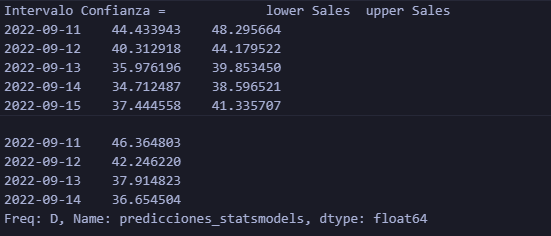
\includegraphics[width=0.5\linewidth]{confianza_sarimax}
	\caption{Intervalo de Confianza y Predicción Arima Manual}
	\label{fig:confianzasarimax}
\end{figure}

La figura muestra la predicciones del modelo SARIMAX junto con las muestras de $test$ reales. El modelo parece ajustarse perfectamente. 
\begin{figure}[!h]
	\centering
	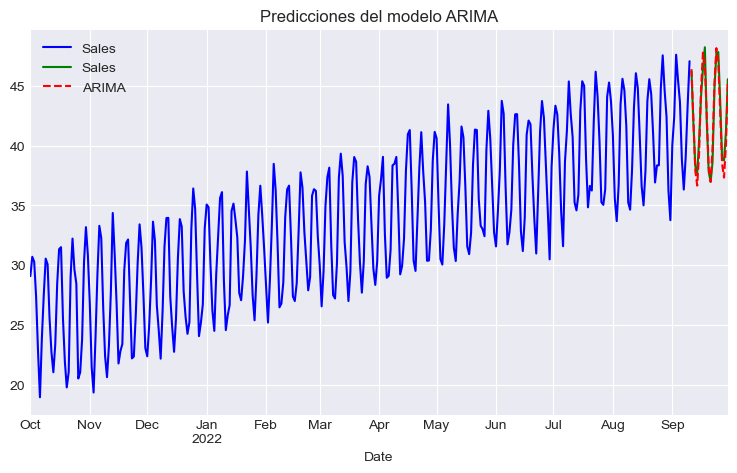
\includegraphics[width=0.7\linewidth]{sarimax}
	\caption{Grafica Arima Manual}
	\label{fig:sarimax}
\end{figure}

\newpage
\subsection{Validación del Modelo}
Al igual que se hizo con el modelo Holt-Winters, con este también se observan los errores producidos entre la predicción y los datos reales.

\begin{figure}[!h]
	\centering
	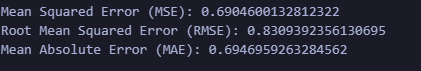
\includegraphics[width=0.7\linewidth]{error_control_sarimax}
	\caption{Errores Arima Manual}
	\label{fig:errorcontrolsarimax}
\end{figure}

Se observa que la los valores obtenidos como errores son muy bajos. Tomando 45 como el promedio de $Sales$ para la predicción, el MSE y MAE dde 0.69 y 0.69 respectivamente indican un error de alrededor del 1.5\%, mientras que el RMSE de 0,83 indica un error de aproximadamente 1.8\%, lo cual es muy cercano al valor obtenido en Holt-Winters.




